\chapter{Design Concepts}
\label{chap:design}

In the this chapter we discuss the platform of choice and the general design of the software components,
involved in the creation of this diploma thesis. We also talk about the database 
design for the back-end server.  
As we mentioned earlier, the main to components are the ELBS viewer and the download portal. 
%In addition, also briefly discuss the integration of a small command-line application to our system, which is used
%for converting scanned images to E-Books for the ELBS viewer.  

\section{Choice of Platform}
\label{chap:Platform}

Early in the design stages we decided to rely heavily on standard tools, protocols and libraries for our project.  
As argued in~\cite[p. 215]{Bloch:2008:EJ}, there are many good reasons for utilizing libraries such as:
\begin{itemize}
	\item	When writing code from scratch, simple things are much easier to get wrong than it initially may seem.
	\item With a pre-implemented library, it is more likely that our code will get faster and more reliable over time,
	as new updates become available.
	\item	When one uses a popular library, the code is in the mainstream of applications.
	\item	Improvement to a library from our side could help others as well.
\end{itemize}

%todo why are libraries important - scalability etc. 
As this is an important part of the project 
in the following sections we present the libraries and techniques we used for the different software components in more detail.

\subsection{ELBS Viewer}
Since we extend the functionality of the ELBS viewer/client, we rely mainly on the libraries and tools that were involved in the creation of the original version ELBS 1.0. First we should note that, the ELBS viewer is a native Windows application and it is written in the C++ programming language. Moreover, we use Qt framework~\cite{wqt} for many of the components of the viewer, such as GUI, networking and others. 

Qt is a cross-platform application development framework that enables the compilation and execution of applications on Windows, Mac OS X, Linux, and different brands of Unix.
A large part of Qt is devoted to providing a platform-neutral interface for everything, ranging
from representing characters in memory to creating a multithreaded graphical application~\cite{bookqt}. In addition to this, Qt offers extensive documentation and online tutorials. However, in our implementation we mainly make use of the Qt framework for its GUI library, which in our option offers   better flexibility and scalability than the standard UI Windows libraries, such as Microsoft Foundation Classes (MFC).  Furthermore,  Qt offers support for many network protocols including the HTTP and the HTTPS protocols, which are used by the ELBS viewer for server communication. Although the Qt framework is platform independent, we only offer a version of the ELBS viewer for Windows. This is due to the fact that we use the Windows DirectDraw API for preventing screenshots. 
A more detailed discussion on this topic can be found in Section~\ref{sec:screenshots}. 
The use of the DirectDraw API was one of the main arguments for the implementation the ELBS viewer 1.0 using 
the C++ programing language. 

Another central feature of Qt is the signals and slots mechanism, which is probably the part  probably the part that differs most from other 
GUI toolkits~\cite{wqtdoc1}. 
Signals and slots are used for communication between objects. Many GUI toolkits use callback functions, e.g. MFC,
 or event listeners, e.g. JAVA Swing. In The signal/slot mechanics of Qt, a signal is emitted when a particular event occurs. For example Qt's widgets have many predefined signals, but one can always subclass widgets to add our own signals to them. A slot is a function that is called in response to a particular signal.
Qt's widgets have many pre-defined slots as well.  
Listing~\ref{listing:qthelloworld} shows a simple \emph{Hello world} GUI program that demonstrates the use of signals and slots. When we click with the mouse on the \verb=QPushButton= a \verb=clicked()= signal is emitted, which is connected to the \verb=quit()= slot of the \verb=QApplication= object by using the static function \verb=QObject::connect()=. As a result, the program
exits. 


Compared to the callback functions, this mechanism has the advantage that it is
type safe, i.e., the signature of a signal must match the signature of the receiving slot; and more importantly that
Qt automatically dismantles a connection if either of the two communicating objects is deleted. This
avoids crashes, and makes the programming process simpler~\cite[Section 1.3]{bookqt}.  

This concludes the brief presentation of some of the features, integrated in the Qt framework. A thorough description of the Qt framework is beyond the scope of this report.
For additional literature on the subject of Qt, we recommend the book~\cite{bookqt}. It
has proven to be very useful information source throughout the development process of the ELBS viewer. 


\subsection{Download Portal Client}
\label{sec:copdp}
In the following section the term client is used to refer to a Web browser.

The download portal is developed as a Web-based application. Web-based systems offer several advantages in comparison to standalone
ones. They minimize the problems of distributing software to users, as well as problems involving hardware and
software compatibility. In addition to this, new releases of systems are immediately available to everyone with Internet access.

There are many different techniques for implementing a Web-based application. They can be
divided into 3 groups: client-side, server-side and
a client-server based approach. 

The client-side solutions consist of a Java applet or a Flash application 
which are downloaded by the browser and then run locally on the computer of the user.
This is achieved by installing a separate browser plug-in. However, this approach has the disadvantage
of requiring a plug-in, which is not always available by default on all Web browsers, and sometimes
installing such plug-ins can only be done by system administrators. This could be a major drawback for the usability ofthe system. 

Server-side solutions  is a centralized architecture, thus all tasks and functions are performed on the server, using popular
programing languages, such as PHP, Perl, Java, or others. 
After their completion a new static HTML page is sent back to the client.
With this approach the client is unable to remember its state and 
every user interaction causes an HTTP round trip over the network, 
requiring browsers to re-render the whole Web page after each request.

The third approach is
a client-server based idea called Asynchronous JavaScript and XML (AJAX),
which is also used by our implementation. 
It works almost the same as the server-side solutions but is more interactive with lower response times. The
reason for this is the fact that some parts of the program logic are moved from the server
to the client, thus not every user interaction necessarily causes a whole new page
to be rendered. Instead with AJAX the client can request 
data from the server in the background, i.e., without the need to freeze the whole user interface. 
This is usually done by XMLHttpRequest API, which is implemented
by the browser. The API can be accessed by the application using JavaScript. It can be
used to handle communication with the server in an asynchronous fashion over a
simple HTTP connection.
This way after the data is received the client can choose to change only a fraction of the Web page.
This, on the other hand, is once again done by JavaScript, which 
can be used to access and manipulate the DOM of the Web page.
An example of an AJAX architecture is illustrated in Figure~\ref{fig:ajax01}.

\begin{figure}[ht]
	\begin{center}
		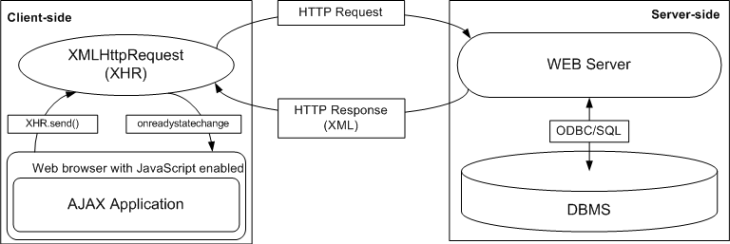
\includegraphics[width=0.8\textwidth]{./img/ajax01a.pdf}
		\caption{Example of an AJAX Architecture}
		\label{fig:ajax01}
	\end{center}
\end{figure}


It should be noted that AJAX has several shortcomings as well. First of all, 
JavaScript must be enabled in the browser, otherwise the application will not start.
However, the developer can
define a specific browser behavior, in case that there is no JavaScript available. It is done by using the
\verb=<noscript>= HTML-tag. 
Nevertheless, the biggest issue with AJAX remains the fact that it is not a
standard. This often requires writing a different code base for different
browsers, and this means less scalability for the application and less productivity for
the developers~\cite{bgwt2}. In the latter case we could avoid some of the issues by using 
Google Web Toolkit (GWT).

GWT is an open source project
and it is developed by Google. It is a set of tools and libraries that allow Web developers to
create AJAX applications in Java. 

The most important component of GWT is the Java-to-JavaScript compiler. It enables the
translation of Java code into highly optimized, browser independent
\footnote{As of GWT version 2.1, GWT supports: 
Firefox 1,~2,~3; Internet Explorer 6,~7,~8; Safari 2~-~5; Opera~9,~10, Chrome 1~-~7, including mobile browsers for Android and the iPhone.} 
JavaScript code.
In addition to this, it provides developers with compile-time error checking. Another
very important aspect of the compiler is the fact that when the code is compiled into
JavaScript, it results in a single JavaScript file for each browser type and target locale.
This is illustrated in Figure~\ref{fig:gwt01}. 
Thus the client downloads and executes only the code that is specifically designed for that platform.  

\begin{figure}[ht]
	\begin{center}
		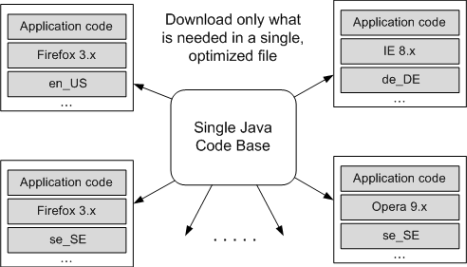
\includegraphics[width=0.8\textwidth]{./img/gwt01a.pdf}
		\caption{GWT Java-to-JavaScript Compiler~\cite[p. 31]{wgio2}}
		\label{fig:gwt01}
	\end{center}
\end{figure}

For additional literature on the subject of GWT, we recommend the book~\cite{bgwt2}. 
 
\subsection{Server-side}
In our approach, we use the Apache Tomcat servlet container, which provides an HTTP server environment for our system. A Tomcat server was also used for ELBS 1.0, which helped us utilize some of the code, written for the previous version of the server. However, we did a lot of refactoring in order to incorporate many new libraries, the  benefit of which is to make our system more scalable and easier to maintain.   
First of all, we rely on the Spring Model View Controller (MVC) Framework~\cite[Chapter 13]{wspring-1}. As the name suggests, the framework 
implements the MVC design pattern. MVC consists of three kinds of objects. The \emph{model} is the application object, the 
\emph{view} is its screen presentation, and the \emph{controller} defines the way the user 
interface  reacts  to  user  input.  Before  MVC,  user  interface  designs  tended  to  lump 
these objects together. MVC decouples them to increase flexibility and reuse~\cite[Section 1.2]{bib:DesignPattern}, which was also the case in ELBS 1.0. Furthermore, in our implementation view objects are constructed using the Apache Tiles Framework~\cite{watiles}, which 
implements the Composite View design pattern~\cite[Chapter 3]{bookj2ee}. With this approach our view objects are created from smaller sub-views, which allows us to reuse the same sub-view for assembling multiple composite views. This makes the view easily configurable, so that changes to the component positioning and look-and-feel could be accomplished more effectively and with a greater ease. Moreover, sub-views are usually described using Java Server Pages (JSP), and the composite views are constructed using a configuration XML file.     

Another very important library that we use is Hibernate. Hibernate facilitates  the storage and retrieval of Java domain objects via Object/Relational Mapping~\cite{whibernate}, which is a technique for converting data from relational databases into Java objects.
Some of the benefits of using Hibernate include:

\begin{itemize}
	\item Hibernate is database independent. In our implementation we use PostgreSQL, but we can easily switch to another database, such as MySQL.
	\item In our case,  Hibernate speeded up the development process, as we did not need to write long and complex SQL queries, but instead worked only with Java objects.
	\item Hibernate offers a number of features to improve the performance of the system as well. For example, it caches objects and manages connections to the database effectively. 
\end{itemize}

In conclusion, we should point out that all libraries we use in our implementation are open source. However, non of their licenses oblige us to release our source code.

\section{System Architecture}
\label{sec:sysarch}
In this section we discuss our general design idea and how the different libraries, described in the previous sections, are utilized by the various software components of our implementation. 

Figure~\ref{fig:architecture} shows the architecture of our system. As can be seen, we have two different clients with a common server.
Both clients communicate with the server only via the HTTP/HTTPS protocol. 
The first client is the ELBS viewer. It is a native Windows application and is
written in the C++ programming language, with the help of the Qt library. The viewer can only display  E-Books, which are provided by the server. Moreover, in our implementation an E-Books is a set of encrypted image files, which reside on the server-side. Each image represents a single page of the book. Pages are sent to the client upon request. 

\begin{figure}[ht]
	\begin{center}
		\includegraphics[width=0.95\textwidth]{./img/architecture.pdf}
		\caption{System Architecture}
		\label{fig:architecture}
	\end{center}
\end{figure}

The second client is the download portal, which is a separate Web-based application and it runs within a browser. The purpose of the download portal is to simplify the process of content distribution to users outside the W�rzburg University. The content is provided by the work-flow system WUEBDIFON and usually refers to scanned images. However, the download portal can distribute any kind of content because of the way it handles documents. A document, in the context of the download portal, is  simply a ZIP file. It is created by the server upon notification from WUEBDIFON. This implies that the document (the zip file) contains all scanned images, and is therefore considered a single entity. For example, a user cannot download only a selected page, he has to download the whole document. We should also mention that, the download portal utilizes some advanced libraries, such as GWT. It offers a more responsive and user-friendly graphical user interface (GUI), which is accomplished by moving some of the program logic from the server to the client.  

On the server-side we can clearly distinguish between the different components of the Spring MVC framework. First, each HTTP request is handled by a single servlet, called \emph{DispatcherServlet}, which 
 dispatches requests to different controllers. Those controllers are mapped to a particular URL in the server configuration. The job of a  controller is to handle the HTTP requests. This task could also involve the use of the Hibernate framework, which is done with the help of different Data Access Objects (DAO). Furthermore, we should mention that our server is capable of accessing remote files with the help of Samba. This means that we do not rely on the operating system to create the necessary samba connections, as they are managed by the server. Accessing remote files is an important task, because scanned images provided by the WUEBDIFON are usually not stored on the local file system of our server. However, we need to access them in order to create the previously mentioned ZIP file.
 
After a controller has finished processing the HTTP request, it creates a \emph{model} object and selects an appropriate view.  By using the Apache Tiles framework, the view and the model are combined 
 into a single HTML page, which is sent back to the client using the DispatcherServlet. 